% chapters/03-system-design.tex
\chapter{Thiết kế hệ thống}\label{chapter_design}

\section{Kiến trúc tổng thể}

Nhatroso Platform được thiết kế theo mô hình Modular Monolith sử dụng ngôn ngữ lập trình Rust. Toàn bộ logic nghiệp vụ được đóng gói trong một API server duy nhất, đảm bảo tính hiệu năng cao, an toàn bộ nhớ \cite{RustBook} và dễ dàng bảo trì. Hệ thống tận dụng nền tảng Loco.rs \cite{LocoRS} (với lõi là Axum \cite{Axum}) để cung cấp các tính năng quản lý cơ sở dữ liệu, xác thực và quản lý background job một cách đồng bộ.

\begin{figure}[htbp]
    \centering
    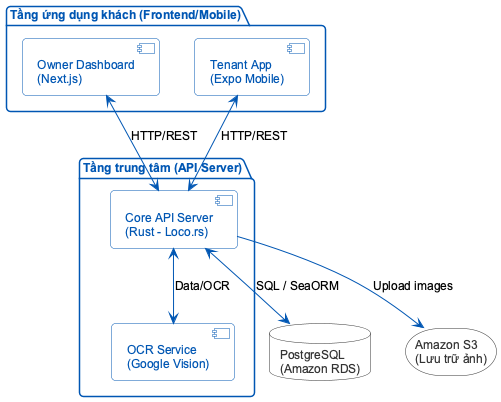
\includegraphics[width=0.85\textwidth]{assets/figures/arch.png}
    \caption{Sơ đồ kiến trúc tổng thể của hệ thống Nhatroso Platform}
    \label{fig:system_architecture}
\end{figure}


Kiến trúc bao gồm các khối chính được quản lý thông qua Docker:

\begin{table}[htbp]
\centering
\caption{Các thành phần hệ thống (Implemented)}
\label{tab:components}
\begin{tabularx}{\textwidth}{llX}
\toprule
\textbf{Thành phần} & \textbf{Công nghệ} & \textbf{Trách nhiệm} \\
\midrule
Owner Dashboard & Next.js 16 & Giao diện quản lý tập trung cho chủ nhà. \\
Tenant Mobile App & Expo (React Native) & Ứng dụng nộp chỉ số và xem hóa đơn cho người thuê. \\
Core API Server & Rust (Loco.rs) & Xử lý logic nghiệp vụ, REST API, RBAC, billing. \\
Database & Amazon RDS (PostgreSQL) & Lưu trữ dữ liệu quan hệ bảo mật cao. \\
Storage & Amazon S3 & Lưu trữ ảnh bằng chứng đồng hồ điện nước. \\
Hosting & Amazon EC2 & Máy chủ thực thi ứng dụng chạy bằng Docker. \\
CI/CD & GitHub Actions & Quản lý pipeline đóng gói và phân phối mã nguồn. \\
Authentication & JWT & Cơ chế xác thực thông qua Access \& Refresh Tokens. \\
\bottomrule
\end{tabularx}
\end{table}

\section{Thiết kế cơ sở dữ liệu}

Cơ sở dữ liệu được quản lý thông qua SeaORM \cite{SeaORM}, sử dụng hệ quản trị cơ sở dữ liệu PostgreSQL \cite{PostgreSQL} để đảm bảo tính nhất quán, bảo mật và hiệu năng cho toàn bộ hệ thống từ môi trường phát triển đến sản xuất. Thiết kế ưu tiên tính toàn vẹn dữ liệu thông qua các ràng buộc khóa ngoại và hệ thống mã định danh duy nhất toàn cầu (UUID).

\subsection{Sơ đồ quan hệ thực thể}

Các thực thể chính được thiết kế để hỗ trợ quy trình billing linh hoạt và có bằng chứng đối soát. Bảng \ref{tab:entities} liệt kê các thực thể cốt lõi trong phiên bản MVP.

\begin{table}[htbp]
\centering
\caption{Các bảng dữ liệu chính (Sơ đồ thực tế)}
\label{tab:entities}
\begin{tabularx}{\textwidth}{lX}
\toprule
\textbf{Bảng} & \textbf{Mô tả và ràng buộc quan trọng} \\
\midrule
\texttt{users} & Thông tin người dùng, \texttt{role} (OWNER/TENANT). ID kiểu UUID. \\
\texttt{buildings} & Thông tin tòa nhà thuộc sở hữu của chủ trọ. \\
\texttt{floors} & Phân cấp tầng trong tòa nhà. \\
\texttt{rooms} & Phòng thuê, trạng thái (VACANT, OCCUPIED, etc.). \\
\texttt{services} & Danh mục dịch vụ (Điện, Nước, Rác, etc.). \\
\texttt{room\_services} & Liên kết các dịch vụ được áp dụng cho từng phòng cụ thể. \\
\texttt{price\_rules} & Quản lý đơn giá theo thời gian hiệu lực cho từng dịch vụ tại mỗi phòng. \\
\texttt{contracts} & Hợp đồng thuê phòng, ràng buộc 01 hợp đồng \texttt{ACTIVE} tại một thời điểm. \\
\texttt{meters} & Thiết bị đo (Đồng hồ điện/nước) gắn với phòng. \\
\texttt{meter\_requests} & Phiên yêu cầu nộp chỉ số theo kỳ (tháng) cho tòa nhà. \\
\texttt{meter\_readings} & Kết quả ghi nhận chỉ số: ảnh bằng chứng, giá trị manual và trạng thái duyệt. \\
\texttt{invoices} & Hóa đơn kỳ của phòng, tính toán dựa trên hợp đồng và chỉ số điện nước. \\
\texttt{invoice\_details} & Chi tiết các khoản mục trong hóa đơn (Label + Amount). \\
\bottomrule
\end{tabularx}
\end{table}

\section{Thiết kế API}

API được triển khai theo chuẩn RESTful với tiền tố \texttt{/api/v1}. Các endpoint được bảo vệ bởi lớp middleware xác thực JWT.

\begin{table}[htbp]
\centering
\caption{Các API endpoint chính}
\label{tab:api}
\begin{tabularx}{\textwidth}{llX}
\toprule
\textbf{Nhóm} & \textbf{Method / Path} & \textbf{Mô tả} \\
\midrule
Auth & POST /auth/login & Đăng nhập và nhận cặp JWT tokens. \\
 & POST /auth/refresh & Sử dụng refresh token để cấp mới access token. \\
\midrule
Property & GET /rooms & Danh sách phòng và trạng thái. \\
 & POST /room-services & Cấu hình dịch vụ áp dụng cho phòng. \\
\midrule
Meters & POST /meter-requests & Khởi tạo kỳ nộp chỉ số cho tòa nhà. \\
 & POST /meter-readings & Tenant nộp chỉ số kèm ảnh chụp từ mobile app. \\
 & PATCH /meter-readings/:id & Owner phê duyệt/từ chối chỉ số thực tế. \\
\midrule
Billing & POST /invoices/calculate & Xem trước giá trị hóa đơn dựa trên chỉ số thực tế. \\
 & POST /invoices & Chốt và phát hành hóa đơn cho kỳ. \\
 & GET /invoices/:id & Truy vấn chi tiết hóa đơn kèm theo line items. \\
\bottomrule
\end{tabularx}
\end{table}

\section{Thiết kế luồng nghiệp vụ quan trọng}

\subsection{Luồng nhận diện tự động và phê duyệt chỉ số}

Hệ thống đã triển khai thành công tính năng trích xuất chỉ số tự động để giảm tải cho cả người thuê lẫn người quản lý:
\begin{enumerate}
  \item Hệ thống tạo \texttt{meter\_requests} hằng tháng hoặc kích hoạt nộp khi có yêu cầu.
  \item Người thuê (Tenant) nhận thông báo và chụp ảnh đồng hồ qua ứng dụng Mobile App.
  \item Ảnh chụp được đẩy lên server, sau đó tương tác với Google Cloud Vision API để thực hiện kỹ thuật OCR nhằm bóc tách chuỗi số và trích xuất chỉ số tự động.
  \item Ảnh bằng chứng được lưu trữ trên Amazon S3 và kết quả trả về được lưu vào Data Model ở trạng thái \texttt{PENDING}.
  \item Chủ nhà (Owner) truy cập Dashboard Web để đối chiếu lại lần cuối và thực hiện \texttt{ACCEPT}.
  \item Chỉ số \texttt{ACCEPTED} trở thành cơ sở tính hóa đơn.
\end{enumerate}

\subsection{Quy trình tính hóa đơn (Billing Logic)}

Logic tính toán được thực hiện tại server Rust để đảm bảo an toàn. Hệ thống truy vấn \texttt{price\_rules} có hiệu lực tại thời điểm tạo hóa đơn, kết hợp với chênh lệch chỉ số giữa hai kỳ liên tiếp.

Hóa đơn được tạo dưới dạng bản nháp (\texttt{calculate}) để owner kiểm tra trước khi phát hành chính thức, đảm bảo tính chính xác tuyệt đối của dữ liệu.

\section{Thiết kế luồng Tích hợp và Triển khai tự động (CI/CD)}

Quy trình phát triển và vận hành (DevOps) được thiết kế hiện đại trên nền tảng GitHub Actions kết hợp chặt chẽ với AWS và Docker:
\begin{enumerate}
    \item \textbf{Continuous Integration (CI):} Bất kỳ thay đổi mã nguồn mới nào khi được đẩy (Push/Merge) lên nhánh chính sẽ kích hoạt quy trình Build mã nguồn Rust tự động, thực hiện kiểm thử (Unit/Integration Testing \cite{RustTesting}) và quét bảo mật mã nguồn. Nếu thành công, mã nguồn được đóng gói ra một Docker Image \cite{Docker} rút gọn.
    \item \textbf{Continuous Deployment (CD):} Docker Image được hệ thống CI tự động đẩy lên Container Registry (như Amazon ECR hoặc Docker Hub). Ngay sau đó tiến trình CD sẽ kích hoạt một lệnh (Webhook/SSH) đến Server Amazon EC2 để tiến hành kéo bản nâng cấp mới về và khởi động lại dịch vụ backend API mà không làm hệ thống ngừng hoạt động (zero-downtime).
\end{enumerate}
